%BEGIN_FOLD PREAMBLE %%%
%%%%%%%%%%%%%%%%%%%%%%%%%%%%%%%%%%%%%%%%%% Don't touch this %%%%%%%%%%%%%%%%%%%%%%%%%%%%%%%%%%%%%%%%%%
\documentclass[11pt]{article}
\usepackage{Z_costumpreamble1}
\usepackage{fancyhdr} % for headers
\addbibresource{Literature.bib}
\pagestyle{fancy}
\fancyhead{}
\fancyfoot{}
\pagestyle{plain} % no page numbers
%%%%%%%%%%%%%%%%%%%%%%%%%%%%%%%%%%%%%%%%%%%%%%%%%%%%%%%%%%%%%%%%%%%%%%%%%%%%%%%%%%%%%%%%%%%%%%%%%%%%%%

%%%%%%%%%%%%%%%%%%%%%%%% Modify Course title, instructor name, semester here %%%%%%%%%%%%%%%%%%%%%%%%%
\title{\vspace{1cm} \relsize{-1}{Seminar DSID0002} \\ \vspace{.25cm} \relsize{2}{Data Management \& Integration}}
\author{Ivo Bantel, Bingjie Cheng, Simon Jantschgi, Yu Zhang\thanks{Alphabetical order; all contributed equally.}}
\date{Handed in: 27.11.2020}
%%%%%%%%%%%%%%%%%%%%%%%%%%%%%%%%%%%%%%%%%%%%%%%%%%%%%%%%%%%%%%%%%%%%%%%%%%%%%%%%%%%%%%%%%%%%%%%%%%%%%%

%%%%%%%%%%%%%%%%%%%%%%%%%%%%%%%%%%%%%%%%%% Don't touch this %%%%%%%%%%%%%%%%%%%%%%%%%%%%%%%%%%%%%%%%%%
\usepackage{Z_costumpreamble2}
%%%%%%%%%%%%%%%%%%%%%%%%%%%%%%%%%%%%%%%%%%%%%%%%%%%%%%%%%%%%%%%%%%%%%%%%%%%%%%%%%%%%%%%%%%%%%%%%%%%%%%

%%%%%%%%%%%%%%%%%%%%%%%%%%%%%%%%%%%%%%%% Modify header here %%%%%%%%%%%%%%%%%%%%%%%%%%%%%%%%%%%%%%%%%%
\fancyhead[L]{HS20}
\fancyhead[C]{}
\fancyhead[R]{}
\fancyfoot[C]{}
%%%%%%%%%%%%%%%%%%%%%%%%%%%%%%%%%%%%%%%%%%%%%%%%%%%%%%%%%%%%%%%%%%%%%%%%%%%%%%%%%%%%%%%%%%%%%%%%%%%%%%

%%%%%%%%%%%%%%%%%%%%%%%%%%%%%%%%%%%%%%%%%% Don't touch this %%%%%%%%%%%%%%%%%%%%%%%%%%%%%%%%%%%%%%%%%%
\usepackage{Z_costumpreamble3}
\usepackage{enumitem}
\setlist{nosep} % compressed lists: fully compressed: nosep; partly compressed: noitemsep
%%%%%%%%%%%%%%%%%%%%%%%%%%%%%%%%%%%%%%%%%%%%%%%%%%%%%%%%%%%%%%%%%%%%%%%%%%%%%%%%%%%%%%%%%%%%%%%%%%%%%%
%END_FOLD PREAMBLE %%%
\begin{document}
    \maketitle
	\begin{tikzpicture}[remember picture,overlay]
        \node[anchor=north west,yshift=-1cm,xshift=1cm] at (current page.north west)
            {
\includegraphics[width=.5\textwidth]{uzh_logo_e_pos_web_main_zone.jpg}};
    \end{tikzpicture}
    \paragraph{} \vspace{-1cm}
		The following documentation gives a brief overview of the data and the undertaken steps. Data and code are available \href{https://github.com/ibantel/DSI_Data-Management-and-Integration_Group6}{here}.
\section*{Process description}
	\paragraph{1. Schemes}
		To start, a relational graph was created as an overview. For this, the entities involved in the four datasets were pinpointed, i.e. participants, questions from the questionnaire task, and tasks from each individual behavioural experiment. Attributes were further assigned to each entity and relationships among the entities were also determined. An ER schema was generated then using the above information. On the basis of the ER schema, the relational graph was generated using ERdplus software. See Figures \ref{fig:ER} \& \ref{fig:relational_schema} for the relational and the ER scheme.
		\begin{figure}[h] % ER scheme
			\centering
			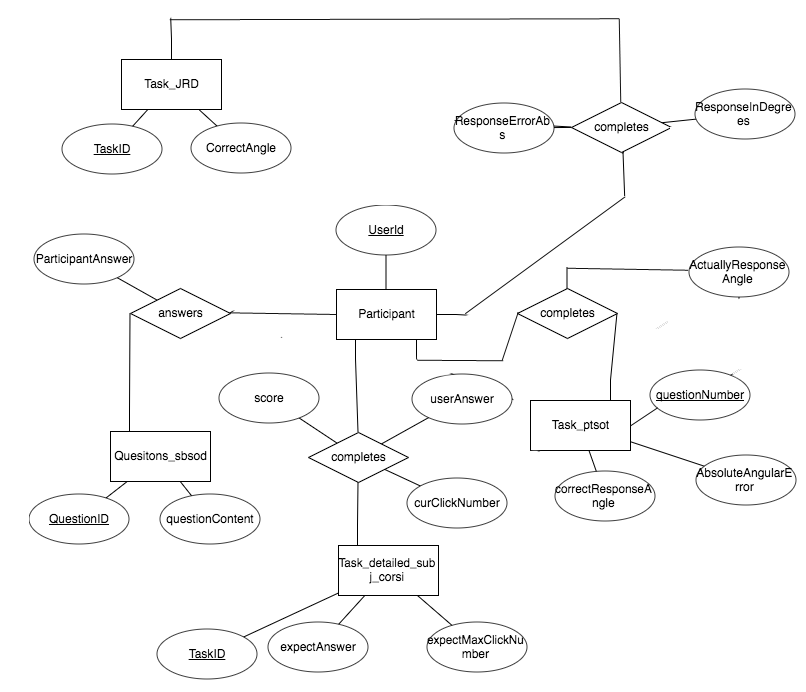
\includegraphics[width=\textwidth]{../organizational-figures/ER diagram_resized.png}
			\caption{ER scheme}
			\label{fig:ER}
		\end{figure}
		\begin{figure}[h] % relational scheme
			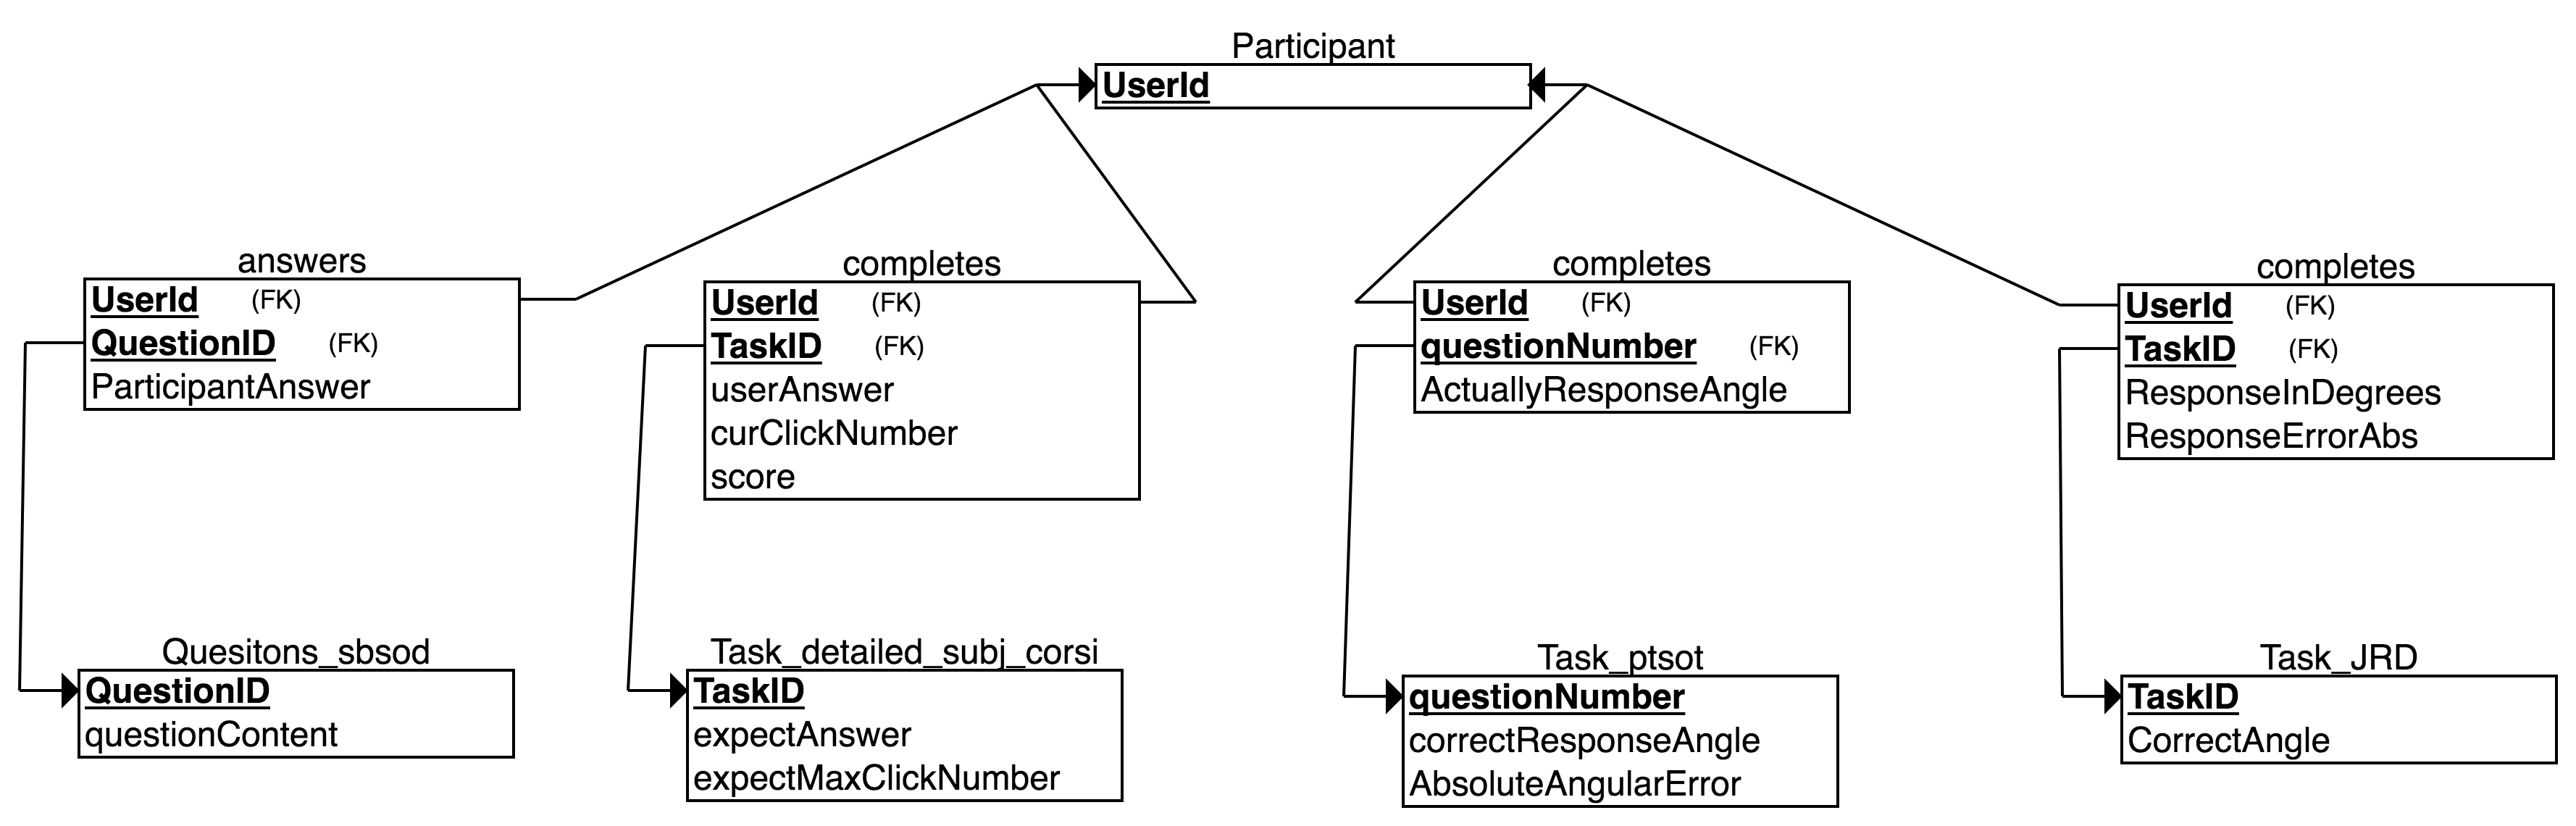
\includegraphics[width=\textwidth]{../organizational-figures/Relational schema.png}
			\caption{Relational scheme}
			\label{fig:relational_schema}
		\end{figure}
	\paragraph{2. Reading in data}
		In the first step of hands-on work, we crawl through the folder structure the data comes in and create a dictionary of paths and files. We then read in the respective data files and combine them into a data frame (using python's \texttt{pandas} module; s. \texttt{1-Data-reading-manipulation.ipynb} in the GitHub repository for details).
	\paragraph{3. Structuring and relating data}
		We relate the different data frames by ensuring they each contain unique IDs identifying them and relating the respective cases according to the ER schema created above.
	\paragraph{4. Export to SQL}
		To make Python interact with the PostgreSQL database, we use two modules from python: \texttt{sqlalchemy} and \texttt{psycopg2}. The \texttt{create\_engine()} call from \texttt{sqlalchemy} recalls an engine configuration. Then we use \texttt{Engine} to provide access to a \texttt{Connection}, which can then invoke SQL statements (with \texttt{engine.connect()} as connection). When python and the SQL database are connected, we use the command: \texttt{pandas.DataFrame.to\_sql()} to export the Python data to SQL.
\newpage
\section*{Data description}
	\paragraph{}
		To give a better impression of the used data, we briefly detail the the four underlying, logically connected data sets below. Unique IDs are underlined.
	\paragraph{\texttt{detailed\_subj\_xx}}
		\begin{itemize}
			\costitem \underline{UserId}: participant ID
			\costitem Correct: 1 = correct, 0 = wrong
			\costitem userAnswer: the answer user provided (the numbers indicates the labels of the squares)
			\costitem expectAnswer: the answer that is expected from the user (correct answer) (the numbers indicates the labels of the squares)
			\costitem curClickNumber: the current number of the squares that user have clicked 
			\costitem expectMaxClickNumber: the max. number of the squares that user should click
		\end{itemize}
	\paragraph{\texttt{ptsot\_results}}
		\begin{itemize}
			\costitem \underline{participant ID}: ID of participant; stored in the file name, not in the file itself
			\costitem questionNumber: number of question
			\costitem correctResponseAngle: correct response to question about angle
			\costitem ActuallyResponseAngle: given response to question about angle
			\costitem AbsoluteAngularError: difference between correct and given response
		\end{itemize}
	\paragraph{\texttt{sbsod}}
		\begin{itemize}
			\costitem \underline{participant ID}: ID of participant; stored in the file name, not in the file itself
			\costitem QuestionID: the ID of the questions. In total 15 questions
			\costitem questionContent: the question presented to the participant
			\costitem ParticipantAnswer: answer given, on a 1-7 likert scale 
		\end{itemize}
	\paragraph{\texttt{UnityDataSave} --- incl. \texttt{JDR} and \texttt{RouteTest}}
		\begin{itemize}
			\costitem \underline{partID}: ID of participant; stored in the file name, not in the file itself
			\costitem City\_mapLMs, StandingAt, LookingAt, LandmarkToMove: content of the questions
			\costitem CorrectAngle: the correct angle (answer that is expected from the user)
			\costitem ResponseInDegrees: participants' answer
			\costitem ResponseErrorAbs: the absolute error between the correct angle and participants' answer			
		\end{itemize}
\end{document}